\documentclass[fr]{../../../../../../eplexam}

\usepackage{ulem}

\renewcommand{\b}[1]{\mathbf{#1}}
\newcommand{\tend}[1]{\oalign{\mbox{\boldmath$#1$}\crcr\hidewidth$\scriptscriptstyle\sim$\hidewidth}}
\renewcommand{\vec}[1]{\uline{#1}}
\newcommand{\matr}[1]{\uuline{#1}}
\DeclareMathOperator{\Difff}{D}
\newcommand{\Dif}{\Difff\!}
\newcommand{\fDif}[2]{\dfrac{\Dif #1}{\Dif #2}}

\hypertitle{Mécanique des Milieux Continus}{5}{MECA}{1901}{2019}{Janvier}{Majeure}
{Thomas Pomponio}
{Issam Doghri et Philippe Chatelain}

\section{Théorie - Partie 1}

\begin{enumerate}
	\item On rappelle quelques notations et définitions du cours sur la cinématique : $\matr{F} = \matr{R} \cdot \matr{U} = \matr{V} \cdot \matr{R}$ ; $\matr{C} = \matr{F}^T \cdot \matr{F}$ ;  $\matr{B} = \matr{F} \cdot \matr{F}^T$.  Dire si chacune des affirmations suivantes est vraie ou fausse, en justifiant à chaque fois la réponse :
	
	\begin{enumerate}

		\item $\matr{C}^{-1} = \matr{R}^T \cdot \matr{B}^{-1} \cdot \matr{R}$ ;
		\item $\matr{B}$ et $\matr{C}$ ont les mêmes valeurs propres ;
		\item $\matr{B}$ et $\matr{C}$ ont les mêmes vecteurs propres.

	\end{enumerate}	
	
	\item On donne l'équation aux dérivées partielles suivantes en coordonnées cartésiennes (où $\gamma$ désigne une constante et $\sigma_{ij}$ une composante du tenseur des contraintes de Cauchy) :	
	
	\begin{equation*}
	\frac{\partial^2 \sigma_{ij}}{\partial x_k \partial x_k}
	+ \frac{1}{1+\gamma} \frac{\partial^2 \sigma_{ll}}{\partial x_i \partial x_j}
	- \frac{\gamma}{1+\gamma} \delta_{ij} \frac{\partial^2 \sigma_{ll}}{\partial x_k \partial x_k}
	=
	-\left( \frac{\partial f_i}{\partial x_j} - \frac{\partial f_i}{\partial x_i}\right)
	\end{equation*}
	
	\begin{enumerate}

		\item Prendre la trace de chaque terme et écrire l'équation obtenue avec deux notations : $(i)$~indicielle, $(ii)$~tensorielle.
		\item Exprimer l'équation tensorielle obtenue en coordonnées cylindriques.

	\end{enumerate}

Remarque : il me semble qu'il y a une erreur dans le membre de droite de l'équation : le premier terme est un tenseur d'ordre deux (deux indices libres, gradient du vecteur $\vec{f}$), le second est un scalaire (pas d'indice libre, divergence du vecteur $\vec{f}$).  J'ai retranscrit l'énoncé qui a été recopié par un autre étudiant et je ne connais pas l'énoncé d'origine.

\end{enumerate}
	
\begin{solution}	

\begin{enumerate}
 \item \nosubsolution
 
 
 
 \item \textbf{Point a}

Remarque : comme le membre de droite de l'équation ne me semble pas correct, je ne développe que celui de gauche.

\begin{equation*}
\begin{split}
& \frac{\partial^2 \sigma_{ll}}{\partial x_k \partial x_k} + \frac{1}{1+\gamma}	\frac{\partial^2 \sigma_{ll}}{\partial x_k \partial x_k} - \frac{\gamma}{1+			\gamma} \delta_{ii} \frac{\partial^2 \sigma_{ll}}{\partial x_k \partial x_k} \\
& = \frac{\partial^2 \sigma_{ll}}{\partial x_k \partial x_k} + \frac{1}{1+\gamma} 	\frac{\partial^2 \sigma_{ll}}{\partial x_i \partial x_i} - \frac{3 \gamma}{1+		\gamma} \frac{\partial^2 \sigma_{ll}}{\partial x_k \partial x_k} \\
& = \left( 1 + \frac{1}{1+\gamma} - \frac{3 \gamma}{1+\gamma} \right) 				\frac{\partial^2 \sigma_{ll}}{\partial x_k \partial x_k} \\
& = 2 \ \frac{1-\gamma}{1+\gamma} \ \frac{\partial^2 \sigma_{ll}}{\partial x_k 		\partial x_k} \ \text{(Point a.i)}\\
& = 2 \ \frac{1-\gamma}{1+\gamma} \ \Delta \left( \text{tr} \ \matr{\sigma} \right) \ \text{(Point a.ii)} \\
& = 2 \ \frac{1-\gamma}{1+\gamma}
\left( \frac{\partial^2 \text{tr} \ \matr{\sigma}}{\partial r^2}
+ \frac{1}{r} \frac{\partial \text{tr} \ \matr{\sigma}}{\partial r}
+ \frac{1}{r^2} \frac{\partial^2 \text{tr} \ \matr{\sigma}}{\partial \theta^2}
+ \frac{\partial^2 \text{tr} \ \matr{\sigma}}{\partial z^2} \right) \ \text{(Point b)}
\end{split} 
\end{equation*}

\end{enumerate}


\end{solution}	

\section{Théorie - Partie 2}

\begin{enumerate}
	\item Lors de l'établissement de la loi de constitution d'un matériau hyper-élastique, nous avons utilisé des axiomes généraux des lois de constitution.  En mentionner deux, les expliquer brièvement ainsi que les simplifications qu'ils entraînent our le matériau hyper-élastique.
	\item On considère le Théorème de Transport de Reynolds sous la forme suivante :
	
	\begin{equation*}
	\fDif{I(t)}{t} = \int_{\Omega(t)} \frac{\partial \Phi}{\partial t} \ dv + \oint_{\partial \Omega(t)}\Phi \ \vec{v} \cdot \vec{\hat{n}} \ ds 
	\end{equation*}	 

	où $\Omega(t)$ est un volume matériel et $\vec{v}$ est le champ de vitesse du milieu.  On demande des réponses succintes aux questions suivantes :
	
	\begin{enumerate}
		\item Qu'est-ce qu'un volume matériel ?
		\item Commentez cette forme du Théorème de Transport de Reynolds.
		\item Qu'est-ce qu'un volume de controle $\Omega_c(t)$ ?
		\item Comment (avec quel argument) a-t-on dérivé la varitation temporelle de la quantité $I_c(t)=\int_{\Omega_c(t)} \Phi\ dv$ lorsqu'elle est intégrée sur le volume de contrôle et non plus sur le volume matériel ?
		\item Donnez un exemple, avec schéma, de l'utilisation d'un volume de contrôle (pour une résolution de problème ou une analyse théorique du cours). 	
	\end{enumerate}
\end{enumerate}


\begin{solution}

\begin{enumerate}
 \item \nosubsolution
 \item \begin{enumerate}[label=(\alph*)]

        \item Un volume qui est constitué des mêmes particules.
        \item Le taux de variation de la quantité $I$ contenue dans le volume matériel est constituée de deux terme : le premier est lié à la variation de $\Phi$ en fonction du temps à $\vec{x}$ fixé (instationnarité du champ), le second est lié au mouvement du milieu matériel (convection). 
        \item Un volume qui peut se déplace indépendamment du milieu matériel.  Au contraire du milieu matériel, il ne comprend donc pas toujours les mêmes particules (les particules du milieu matériel entrent et sortent du volume du contrôle, en fonction des déplacements du volume de contrôle et du milieu matériel).
        \item Les formules utilisées pour un volume matériel font intervenir la vitesse des particules contenue dans le volume de matériel.  On peut généraliser et utiliser les formules avec un champ de vitesse quelconque.  Si on calcule la dérivée sur un volume de contrôle, le champ de vitesse à prendre en compte est celui des points qui définissent le volume de contrôle (ces points ne correspondent alors plus nécessairement à des particules, mais ce sont des coordonnées qui indiquent la position du volume de contrôle.)
        \item Calcul de la poussée d'un réacteur d'avion.  Schéma dans les transparents du cours. 

        \end{enumerate}

\end{enumerate}

\end{solution}


\section{Exercice 1}

On considère une transformation uniforme définie par son gradient de déformation dans un repère orthonormé fixe $(O, \hat{e}_1, \hat{e}_2, \hat{e}_3)$ comme suit :

\begin{equation*}
F_{11}(t) = f(t) \ \text{cos} (\omega t) \ ; \ 
F_{22}(t) = f(t) \ ;  \
F_{33}(t) = 1 \ ;  \
F_{12}(t) = f(t) \ \cos (\omega t)
\end{equation*}

Toutes les autres composantes $F_{ij}(t)$ étant nulles.  On désigne par $\omega \geq 0$ une constante donnée, $t \geq 0$ le temps, et $f(t)$ une fonction continue dérivable qui vérifie : $f(0)=1$ et $f(t)>0, \ \forall \ t>0$.

On limite l'étude au cas : $(\omega t) \in [0;\frac{\pi}{2}[$.

\begin{enumerate}
	\item Calculer la matrice représentant le gradiant de vitesse $L=\left( \nabla \vec{v} \right)^T$, le taux de déformation $\matr{D}$ et le tourbillon ("spin") $\matr{\Omega}$.
\end{enumerate}
	
Pour toute la suite, on considère un modèle de comportement dit hypo-élastique qui est décrit par l'équation suivante :

\begin{equation*}
\dot{\matr{\sigma}} + \matr{\sigma} \cdot \matr{\Omega} - \matr{\Omega} \cdot \matr{\sigma} = \lambda \ \text{tr} (\matr{D}) \matr{I} + 2 \mu \matr{D}
\end{equation*}

où on désigne par $\lambda > 0$ et $\mu > 0$ des constantes matérielles, $\matr{I}$ le tenseur identité d'ordre 2, $\matr{\sigma}$ le tenseur de Cauchy et $\dot{\matr{\sigma}}= \text{D} \matr{\sigma} \ / \ \text{D}t$ sa dérivée particulaire (ou temporelle totale).  

\begin{enumerate}
\setcounter{enumi}{1}
	\item Donner l'expression de $\dot \sigma_{ij}(t)$ en fonction des données $(t, \ f(t), \ \omega, \ \lambda, \ \mu)$.
	\item Donner l'expression de $\text{tr} \ \matr{\sigma}(t)$ en fonction des données.  On suppose que $\sigma_{ij}(0)=0$.  Indications :
	
	\begin{enumerate}
		\item Une primitive de $\frac{g'(x)}{g(x)}$ est : $\ln{\left( g(x)\right)}$ ;
		\item Une primitive de $\tan(x)$ est : $-\ln \left(|\cos(x)| \right)$ ;
		\item On n'a pas besoin de calculer la primitive de $\sigma_{12}(t) \frac{\omega}{\cos(\omega t)}$.
	\end{enumerate}		
	
	\item Ré-exprimer $\text{tr} \ \matr{\sigma}(t)$ en fonction de $\lambda$, $\mu$ et $\text{det} \ \matr{F}(t)$ uniquement.
	
	\item Que vaut $\text{tr} \ \matr{\sigma}(t)$ quand $\mu$ et $\text{det} \ \matr{F}(t)=1$~?  Interpréter le résultat.
	 
\end{enumerate}

On considère à présent le cas particuler $\omega=0$.

\begin{enumerate}
\setcounter{enumi}{5}

	\item Donner les expression de $\sigma_{ij}(t)$ en fonction des données.  On suppose que $\sigma_{ij}(0)=0$.
	
	\item Dessiner les cercles de Mohr et calculer la contrainte de cisaillement maximale.
	
	\item \textbf{Bonus :} Calculer l'angle entre chaque facette où la contrainte de cisaillement maximale est atteinte et l'axe $(O, \ \vec{\hat{e}_1})$.

\end{enumerate}

\begin{solution}

\begin{enumerate}
 \item 
 
 Le gradient de la vitesse et le gradient de la déformation sont liés par les relations suivantes :

\begin{equation*}
\fDif{\matr{F}}{t} = \matr{L} \cdot \matr{F} \ \ \text{ou} \ \ \matr{L} = \fDif{\matr{F}}{t} \cdot \matr{F}^{-1}
\end{equation*}

Si on ne se souvient plus de la formule, on peut la retrouver en calculant la dérivée particulaire de $\matr{F}$ et en utilisant les définitions des différents tenseurs et vecteurs vues au cours :

\begin{equation*}
\begin{split}
\left( \fDif{\matr{F}}{t} \right)_{ij}
& = \left( \frac{\partial \matr{F}}{\partial t} \right)_{ij}
= \frac{\partial}{\partial t} \left( \frac{\partial x_i}{\partial X_j} \right)
= \frac{\partial}{\partial X_j} \left( \frac{\partial x_i}{\partial t} \right)
= \frac{\partial V_i}{\partial X_j}
= \frac{\partial V_i}{\partial x_p} \ \frac{\partial x_p}{\partial X_j} \\
& = \left( \matr{grad} \ \vec{V} \right)_{ip} \ \left( \matr{F} \right)_{pj}
= \left[ \left( \matr{grad} \ \vec{V} \right) \cdot \matr{F} \right]_{ij}
= \left( \matr{L} \cdot \matr{F} \right)_{ij}
\end{split}
\end{equation*}

La première égalité vient du fait que le gradient de la déformation $\matr{F}$ est une fonction de $\vec{X}$ et de $t$ : comme la dérivée particulaire est par définition la dérivée à $\vec{X}$ fixé, la dérivée particulaire de $\matr{F}$ est égale à la dérivée partielle de $\matr{F}$ par rapport à $t$.  Pour la seconde égalité, on utilise la définition de $\matr{F}$.  Pour la cinquième, on fait appel au fait que $\vec{x}$ est une fonction de $\vec{X}$ et on applique une dérivée en chaîne.

$\matr{F} = \begin{pmatrix} 
f \ \cos(\omega t) & f \ \sin(\omega t) & 0 \\
0 & f & 0 \\
0 & 0 & 1 \\  
\end{pmatrix}$

$\matr{F}^{-1} = \frac{1}{f^2 \ \cos(\omega t)} \
\begin{pmatrix} 
f & -f \ \sin(\omega t) & 0 \\
0 & f \ \cos(\omega t) & 0 \\
0 & 0 & f^2 \ \cos(\omega t) \\  
\end{pmatrix}$ 

$\fDif{\matr{F}}{t} =
\begin{pmatrix} 
f' \ \cos(\omega t)-f \omega \ \sin(\omega t) & f' \ \sin(\omega t) + f \omega \ \cos(\omega t) & 0 \\
0 & f' & 0 \\
0 & 0 & 0 \\  
\end{pmatrix}$ 

$\boxed{ \matr{L} =
\begin{pmatrix} 
\frac{f'}{f}-\omega \ \tan(\omega t) & \frac{\omega}{\cos (\omega t)} & 0 \\
0 & \frac{f'}{f} & 0 \\
0 & 0 & 0 \\  
\end{pmatrix} }$ 

$\boxed{ \matr{D}
= \frac{1}{2} \left( \matr{L} + \matr{L}^T \right)
= \begin{pmatrix} 
\frac{f'}{f}-\omega \ \tan(\omega t) & \frac{\omega}{2 \ \cos (\omega t)} & 0 \\
\frac{\omega}{2 \ \cos (\omega t)} & \frac{f'}{f} & 0 \\
0 & 0 & 0 \\  
\end{pmatrix} }$ 

$\boxed{ \matr{\Omega}
= \frac{1}{2} \left( \matr{L} - \matr{L}^T \right)
= \begin{pmatrix} 
0 & \frac{\omega}{2 \ \cos (\omega t)} & 0 \\
- \frac{\omega}{2 \ \cos (\omega t)} & 0 & 0 \\
0 & 0 & 0 \\  
\end{pmatrix} }$

Vérification des calculs : $\matr{D}$ est bien symmétrique et $\matr{\Omega}$ est bien anti-symmétrique.
 
 \item 
 
Il faut calculer les composantes du tenseur :

\begin{equation*}
\dot{\matr{\sigma}} = \lambda \ \text{tr} (\matr{D}) \matr{I} + 2 \mu \matr{D} - \matr{\sigma} \cdot \matr{\Omega} + \matr{\Omega} \cdot \matr{\sigma}
\end{equation*}

Calcul des différents termes du membre de droite :

$\lambda \ \text{tr} (\matr{D}) = 2 \ \lambda \ \frac{f'}{f} - \lambda \ \omega \ \tan(\omega t)$

$\matr{\sigma} \cdot \matr{\Omega}
= \begin{pmatrix}
-\frac{1}{2} \sigma_{12} \frac{\omega}{\cos(\omega t)} & \frac{1}{2} \sigma_{11} \frac{\omega}{\cos(\omega t)} & 0 \\
-\frac{1}{2} \sigma_{22} \frac{\omega}{\cos(\omega t)} & \frac{1}{2} \sigma_{21} \frac{\omega}{\cos(\omega t)} & 0 \\
-\frac{1}{2} \sigma_{32} \frac{\omega}{\cos(\omega t)} & \frac{1}{2} \sigma_{31} \frac{\omega}{\cos(\omega t)} & 0 \\
\end{pmatrix}$


$\matr{\Omega} \cdot  \matr{\sigma} 
= \begin{pmatrix}
\frac{1}{2} \sigma_{21} \frac{\omega}{\cos(\omega t)} & \frac{1}{2} \sigma_{22} \frac{\omega}{\cos(\omega t)} & \frac{1}{2} \sigma_{23} \frac{\omega}{\cos(\omega t)} \\
-\frac{1}{2} \sigma_{11} \frac{\omega}{\cos(\omega t)} & -\frac{1}{2} \sigma_{12} \frac{\omega}{\cos(\omega t)} & -\frac{1}{2} \sigma_{13} \frac{\omega}{\cos(\omega t)} \\
0 & 0 & 0 \\
\end{pmatrix}$

On additionne les composantes des trois tenseurs.  Vu la longueur des expressions, on écrit les composantes sous forme d'une liste, et pas de matrice :

\begin{tabular}{|l|}
\hline
\rule{0pt}{0pt}
$\dot \sigma_{11} = 2 \ (\lambda+\mu) \frac{f'}{f} - (\lambda+2 \mu) \omega \tan(\omega t) + \sigma_{12} \frac{\omega}{\cos(\omega t)}$ \\
$\dot \sigma_{12} = 2 \ (\mu - \frac{\sigma_{11}}{2} + \frac{\sigma_{22}}{2}) \frac{\omega}{\cos(\omega t)}$ \\
$\dot \sigma_{13} = \frac{1}{2} \sigma_{23} \frac{\omega}{\cos(\omega t)}$ \\
$\dot \sigma_{21} = \dot \sigma_{12}$ \\
$\dot \sigma_{22} = 2 \ (\lambda+\mu) \frac{f'}{f} - \lambda \ \omega \tan(\omega t) - \sigma_{12} \frac{\omega}{\cos(\omega t)}$ \\
$\dot \sigma_{23} = - \frac{1}{2} \sigma_{13} \frac{\omega}{\cos(\omega t)}$ \\
$\dot \sigma_{31} = \dot \sigma_{13}$ \\
$\dot \sigma_{32} = \dot \sigma_{23}$ \\
$\dot \sigma_{33} = 2 \ \lambda \ \frac{f'}{f} - \lambda \ \omega \tan(\omega t)$ \\
\hline 
\end{tabular}

Ici, on a déduit $\dot \sigma_{21} = \dot \sigma_{12}$, $\dot \sigma_{31} = \dot \sigma_{13}$ et $\dot \sigma_{32} = \dot \sigma_{23}$ du fait que $\matr{\sigma}$ est symmétrique.  On pourrait calculer ces composantes, pour vérifier que ce soit bien le cas et que l'on ne s'est pas trompé dans les calculs.
 
 \item 
 
Attention ! Je ne suis pas certain que la méthode employée soit correcte.  Le résultat me semble correct car il fait appel aux indications données dans l'énoncé, mais je ne sais pas si le raisonnement est rigoureux.  Je propose quand même ce que j'ai trouvé et je vous indiquerai où le raisonnement me semble poser problème.

On cherche d'abord en lien entre la trace de $\matr{\sigma}$ et celle de $\dot {\matr{\sigma}}$ :

\begin{equation*}
\text{tr} \ \dot{\matr{\sigma}}
= \dot{\sigma_{ii}}
= \fDif{\sigma_{ii}}{t}
= \fDif{\ \text{tr} \ \matr{\sigma}}{t}
\end{equation*}

On peut donc trouver $\text{tr} \ \matr{\sigma}$ en intégrant $\text{tr} \ \dot{\matr{\sigma}}$, ce qui ne demande que d'intégrer la somme des éléments diagonaux calculés au point précédent.  Problème : comment intégrer la dérivée particulaire~?  On retourne à sa définition.  Pour la composante $\sigma_{ij}$, on a  :

\begin{equation*}
\begin{split}
\fDif{\sigma_{ij}(\vec{x}, \ t)}{t}
& = \left( \frac{\partial \sigma_{ij}(\vec{x}, t)}{\partial t} \right)_{\vec{X}} \\
& = \left( \frac{\partial \sigma_{ij}}{\partial t} \right)_{\vec{x}} + \left( \frac{\partial \sigma_{ij}}{\partial x_i} \right)_{t} \ \left( \frac{\partial x_i}{\partial t} \right)_{\vec{X}} \\
& = \frac{\partial \sigma_{ij}}{\partial t} + \left( \vec{grad} \ \sigma_{ij} \right) \cdot \vec{V}
\end{split}
\end{equation*}

C'est ici que j'ai un doute sur le raisonnement : nous avons vu au cours que $\matr{\sigma}$ est fonction de $\vec{x}$, $\vec{\hat{n}}$ et $t$.  Ici, puisque les composantes de $\dot{\matr{\sigma}}$ obtenues au point précédent ne dépendent pas de $\vec{x}$, je suppose qu'il en est de même pour celles de $\matr{\sigma}$, car si $\vec{x}$ intervenait dans les composantes de $\matr{\sigma}$, il n'aurait pas disparu en dérivant par rapport à $t$.  Si ceci est bien correct, on a $\vec{grad} \ \sigma_{ij} = \vec{0}$ et la dérivée particulaire est égale à la dérivée partielle par rapport au temps.  On peut donc calculer les composantes $\sigma_{ij}$ en intégrant les $\dot{\sigma}_{ij}$ par rapport à $t$ sans se soucier de la position $\vec{x}$ ou $\vec{X}$.

\begin{equation*}
\begin{split}
\text{tr} \ \matr{\sigma}
& = \int \dot{\matr{\sigma}} \ \text{d}t \\
& = \int \left[ (6\lambda+4\mu)\frac{f'}{f} - (3\lambda+2\mu) \ \omega \tan (\omega t) \right] \ \text{d}t \\
& = (6\lambda+4\mu) \ \text{ln} \left( f(t) \right) + (3\lambda+2\mu) \ \ln \left(|\cos(\omega t)| \right) + K
\end{split}
\end{equation*}

Remarque : on peut directement écrire $\text{ln} \left( f(t) \right)$ car $f(t)>0, \ \forall \ t>0$.

On applique les conditions initiales :

En $t=0$ : $\sigma_{ij}=0$ et $f(0)=1$.

$ \Rightarrow \ \text{tr} \ \matr{\sigma} = 0 = (6\lambda+4\mu) \ \text{ln} \left( f(0) \right) + (3\lambda+2\mu) \ \ln \left(|\cos(0)| \right) + K$

$\Rightarrow \ K = 0$

$\Rightarrow \ \boxed{ \text{tr} \ \matr{\sigma} = (6\lambda+4\mu) \ \text{ln} \left( f(t) \right) + (3\lambda+2\mu) \ \ln \left(|\cos(\omega t)| \right) }$


\item 

\begin{equation*}
\begin{split}
\text{tr} \ \matr{\sigma}
& = (6\lambda+4\mu) \ \text{ln} \left( f(t) \right) + (6\lambda+4\mu) \ \ln \left(|\cos(\omega t)| \right) \\
& = (3\lambda+2\mu) \ \text{ln} \left( f(t)^2 \right) + (3\lambda+2\mu) \ \ln \left(|\cos(\omega t)| \right) \\
& = (3\lambda+2\mu) \ \text{ln} \left( f(t)^2 |\cos(\omega t)| \right) \\
& = (3\lambda+2\mu) \ \text{ln} \left( f(t)^2 \cos(\omega t) \right) \ \text{car on limite l'étude du cas à } (\omega t) \in [0;\frac{\pi}{2}[ \\
& = (3\lambda+2\mu) \  \text{ln} \left( \text{det} \ \matr{F} \right) \ \text{car } f(t)^2 \cos(\omega t) = \text{det} \ \matr{F} \ \text{(voir \matr{F} à la sous-question 1)}
\end{split}
\end{equation*}

$\Rightarrow \ \boxed{ \text{tr} \ \matr{\sigma} = (3\lambda+2\mu) \  \text{ln} \left( \text{det} \ \matr{F} \right) }$

 \item 
 
Si $\text{det} \ \matr{F} = 1$, $\text{tr} \ \matr{\sigma} = 0$.

Je ne suis pas certain de l'interprétation à donner.  J'indique quand même ce que je pense, et je signale là où je ne suis pas sûr.

\begin{enumerate}
\item $\text{det} \ \matr{F} = J(\vec{\chi}) = \frac{\text{d}v}{\text{d}v_0} = \text{dilatation relative d'un volume élementaire.}$
\item $\text{det} \ \matr{F} = 1$ signifie donc un mouvement isochore.
\item Comment faire le lien avec le fait que $\text{tr} \ \matr{\sigma} = 0$~?  C'est là que je coince~...  Si le mouvement se faisait sans déformation, on pourrait admettre que les contraintes soient nulles.  Mais un mouvement isochore ne signifie pas qu'il n'y a pas de déformation (pensez au cisaillement simple vu au cours : le cube se déforme et devient un "parallélogramme", mais son volume est conservé).  Donc, la seule explication que je vois, c'est que dans notre application, les contraintes ne sont pas liées aux déformations.  Mais je trouve ça vraiment très, très bizarre : cela voudrait dire que le solide n'offre aucune résistance à la déformation, et donc qu'il n'y aurait pas de cohésion entre les particules qui le composent.  Cela ne correspond pas à la description d'un solide.
\item Je me demande donc s'il ne faut pas chercher une explication qui fait intervenir des formules vues au cours, pour démontrer mathématiquement que le résultat est logique.  Mais ne vois pas quelles formules pourraient aider car ce que l'on a vu, c'est 1) des relations générales dans un premier temps et 2) le cas particuler du solide élastique et isotrope.  Or, ici on a un solide, hypo-élastique.
\end{enumerate}
 
 \item 
 
On reprend les expressions des $\sigma_{ij}$ trouvées au point 2, on fait $\omega = 0$, on intègre par rapport au temps, on calcule les constantes d'intégration avec la condition initiale $\matr{\sigma}(t=0)=0$ et on trouve :

$\boxed { \matr{\sigma} =
\begin{pmatrix}
2 \ (\lambda+\mu) \ \text{ln} \left( f(t) \right) & 0 & 0 \\
0 & 2 \ (\lambda+\mu) \ \text{ln} \left( f(t) \right) & 0 \\
0 & 0 & 2 \ \lambda \ \text{ln} \left( f(t) \right) \\
\end{pmatrix} }$

\item 

$ \boxed{ \sigma_1 = \sigma_2 = 2 \ (\lambda+\mu) \ \text{ln} \ \left( f(t) \right)$ et $\sigma_3 = 2 \ \lambda \ \text{ln}  \left( f(t) \right) }$

Remarque : les contraintes principales sont définies telles que $\sigma_1 > \sigma_2 > \sigma_3$.  Dans l'énoncé, on précise : $f(t)>0, \ \forall \ t>0$.  $\text{ln}  \left( f(t) \right)$ est donc défini, mais on ne sait pas s'il est positif ou négatif.  Pour ça, il faudrait savoir si $f(t)$ est supérieure ou inférieure à un.    Pour ordonner les contraintes principales, j'ai fait l'hypothèse que $\text{ln}  \left( f(t) \right) > 0$.

\begin{center}
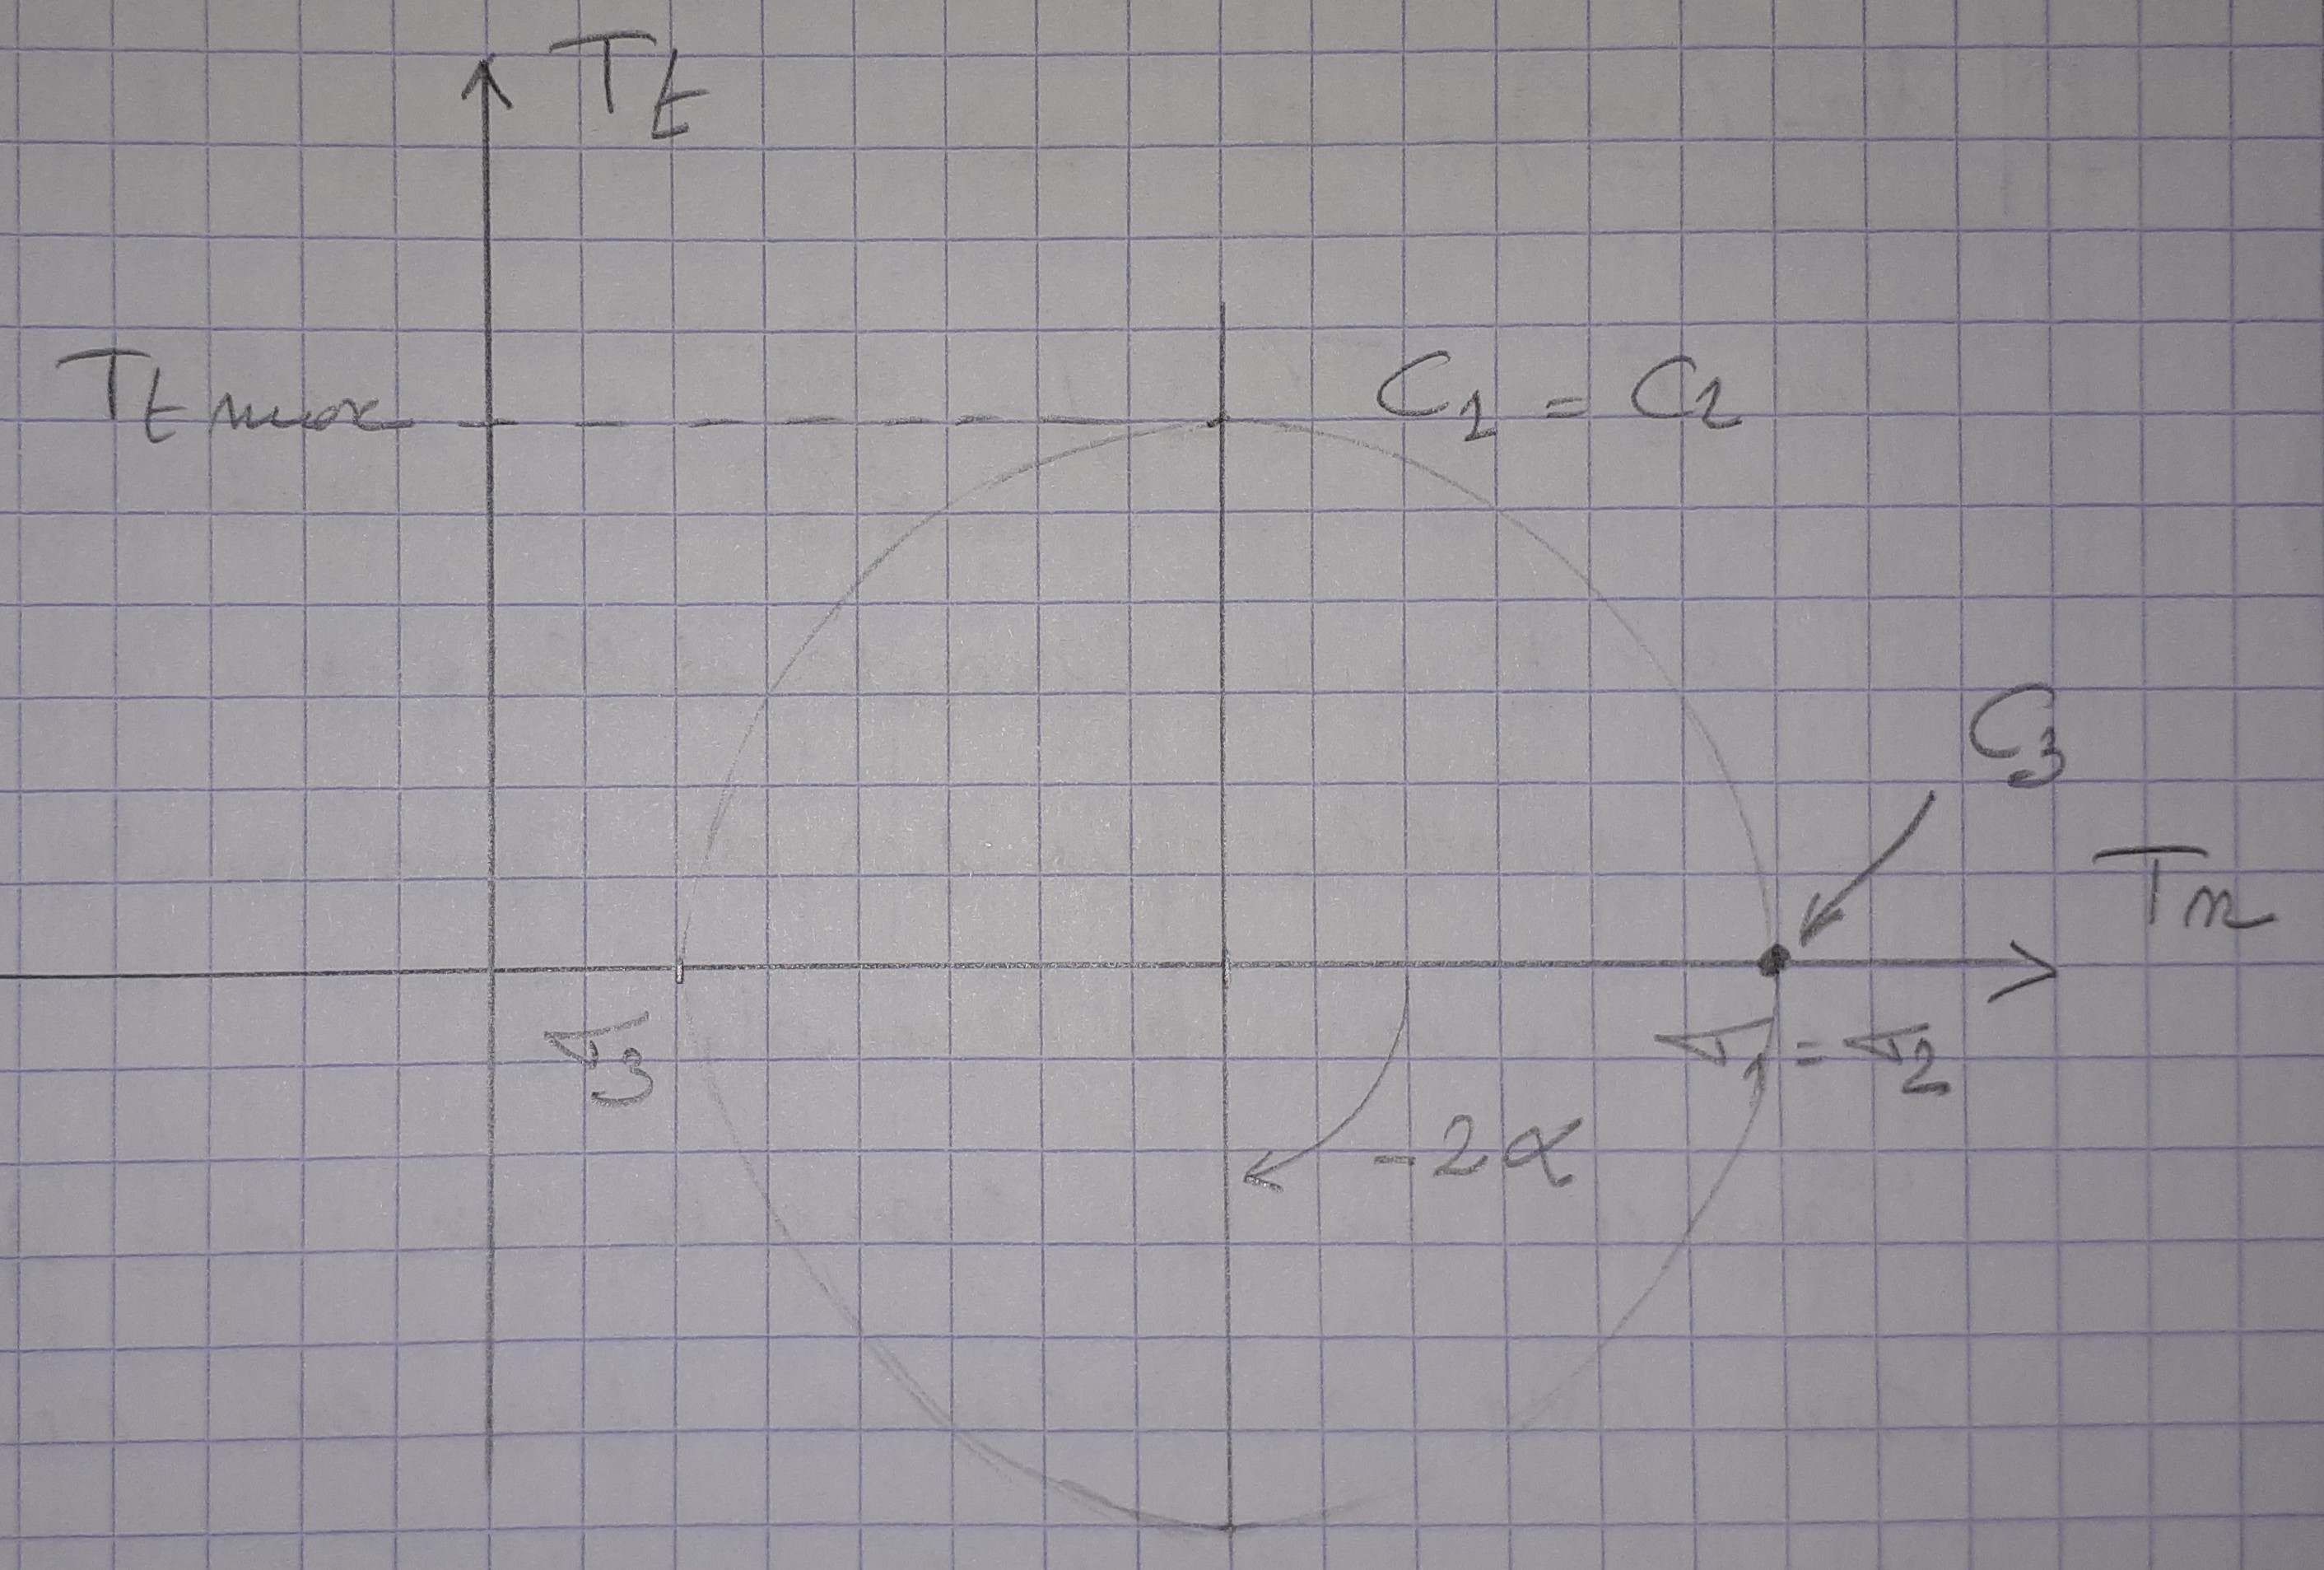
\includegraphics[width=0.9\textwidth]{MMC_Janvier_2019_Maj_Q3_Image1.jpg}
\end{center}

$ \boxed{ T_{t \ max} = \frac{\sigma_1 - \sigma2}{2} = \mu \ \text{ln} \left( f(t) \right) }$

\item 

\begin{center}
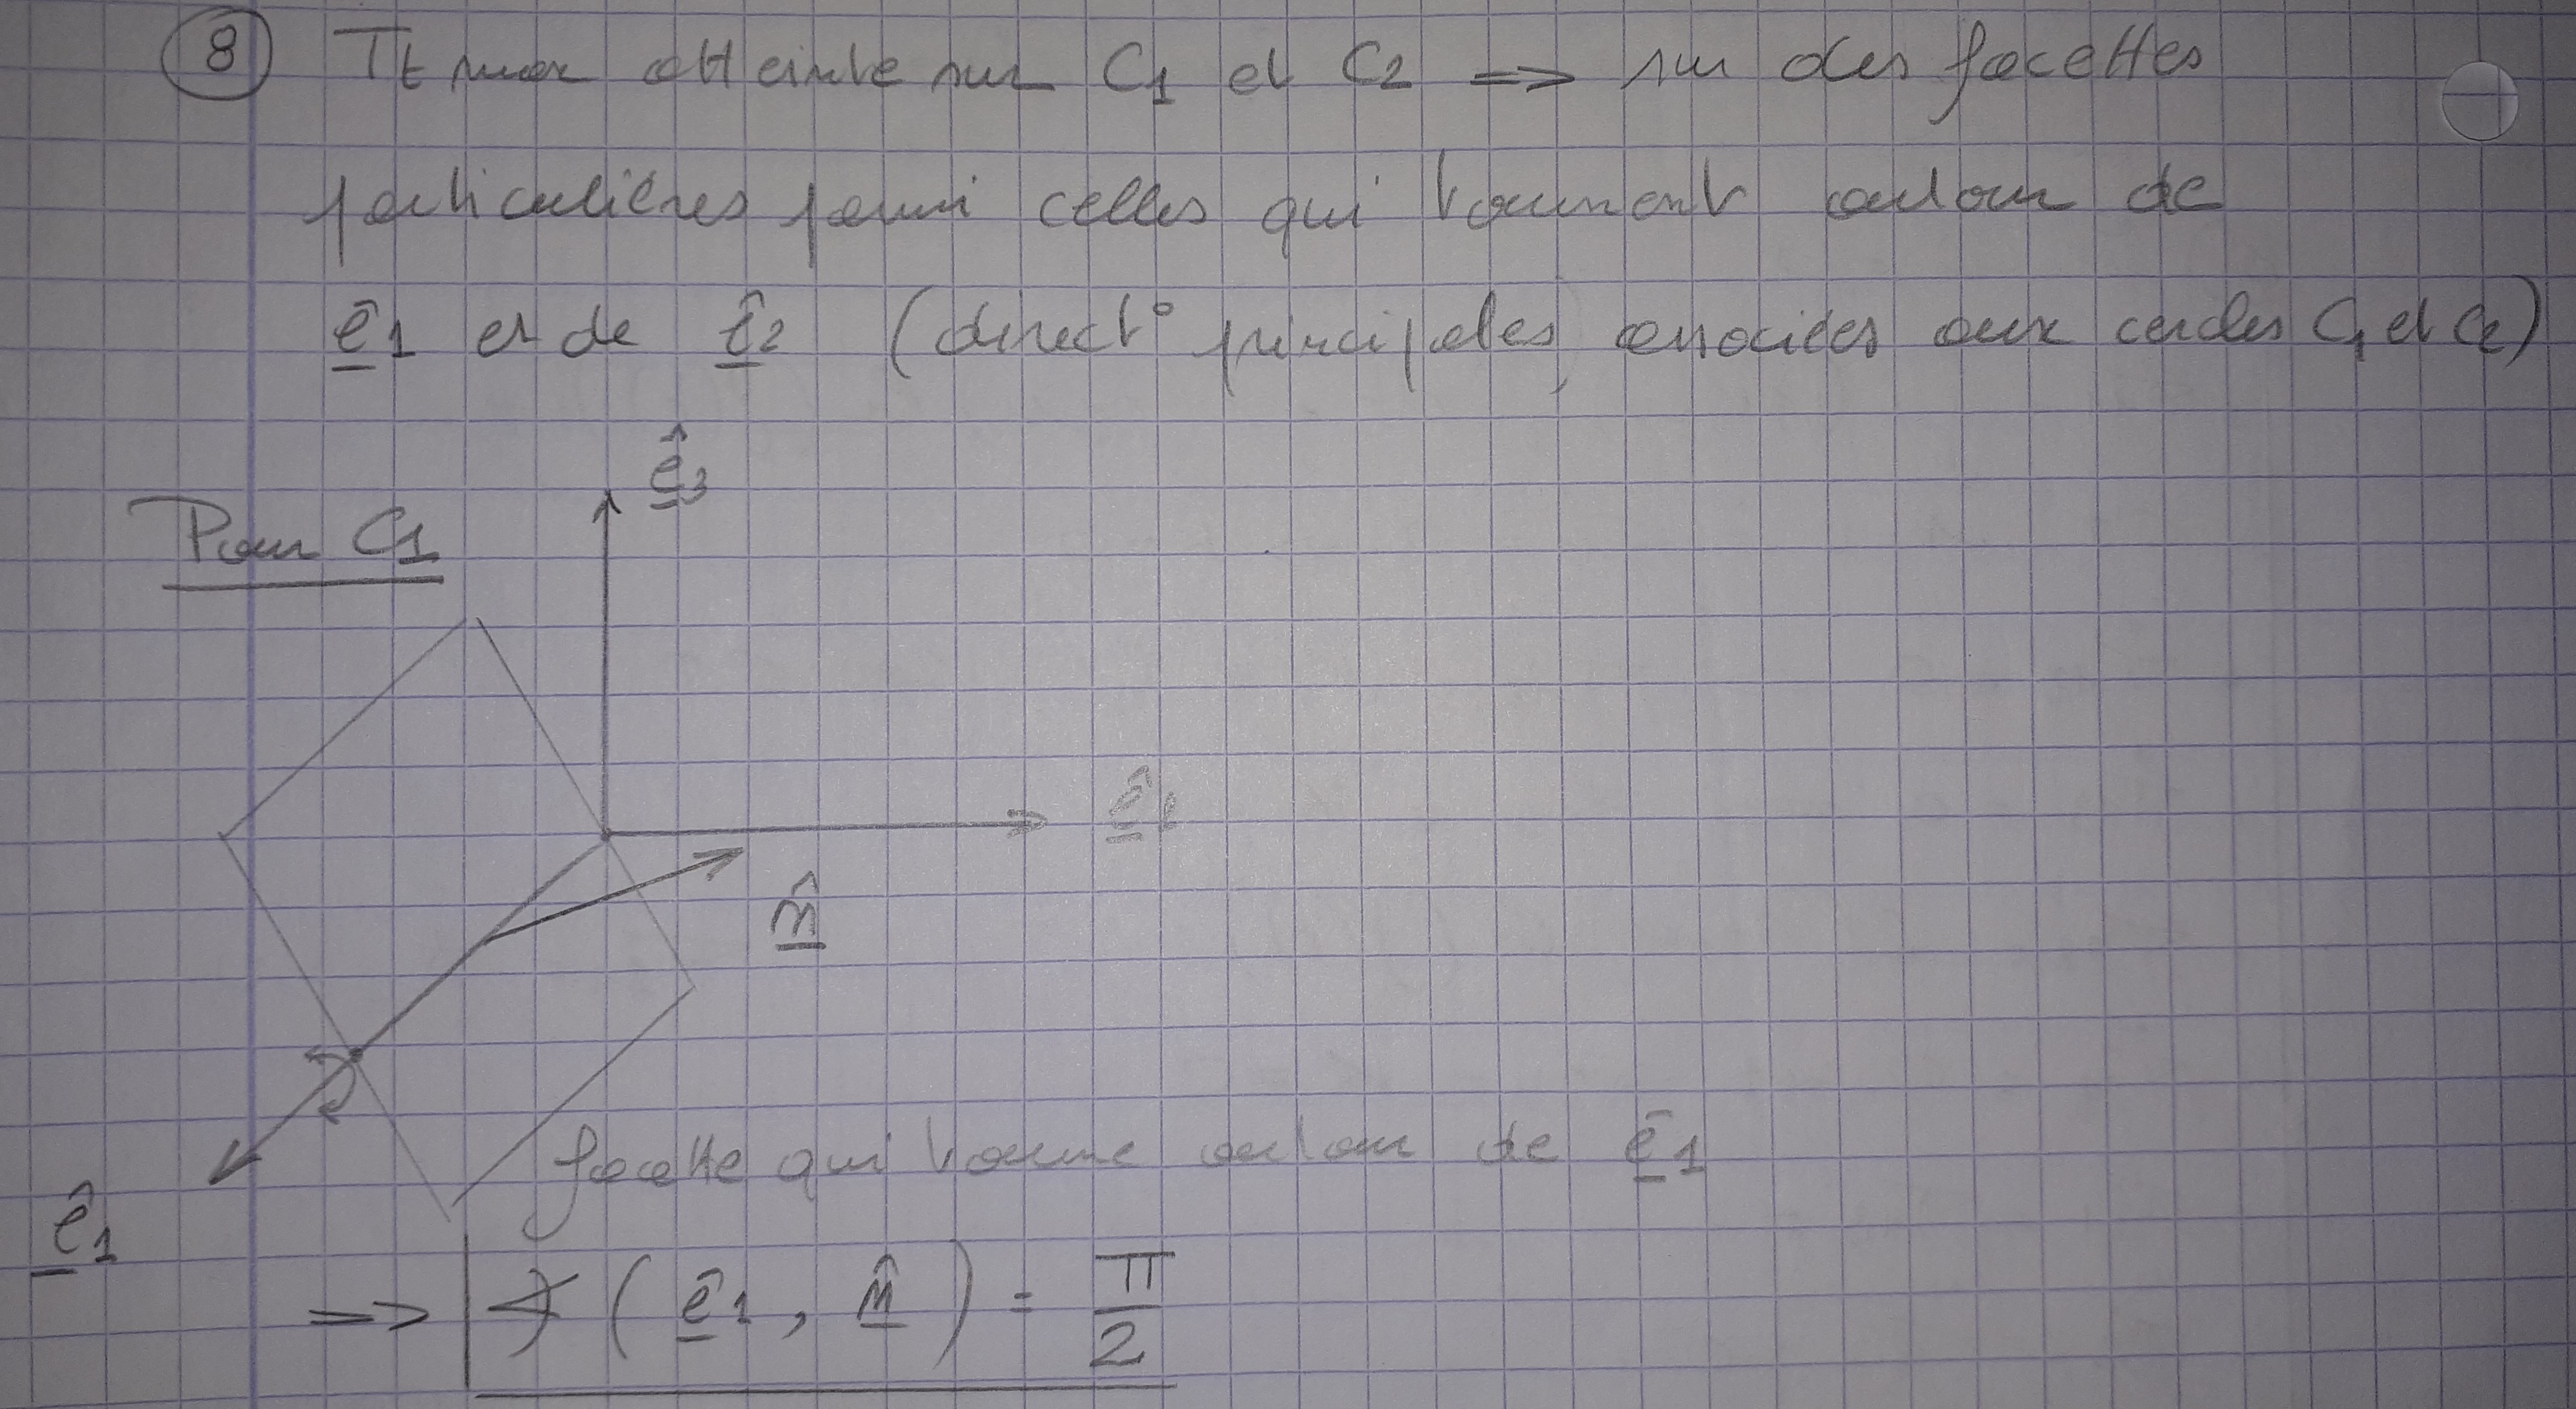
\includegraphics[width=0.9\textwidth]{MMC_Janvier_2019_Maj_Q3_Image2.jpg}
\end{center}

\begin{center}
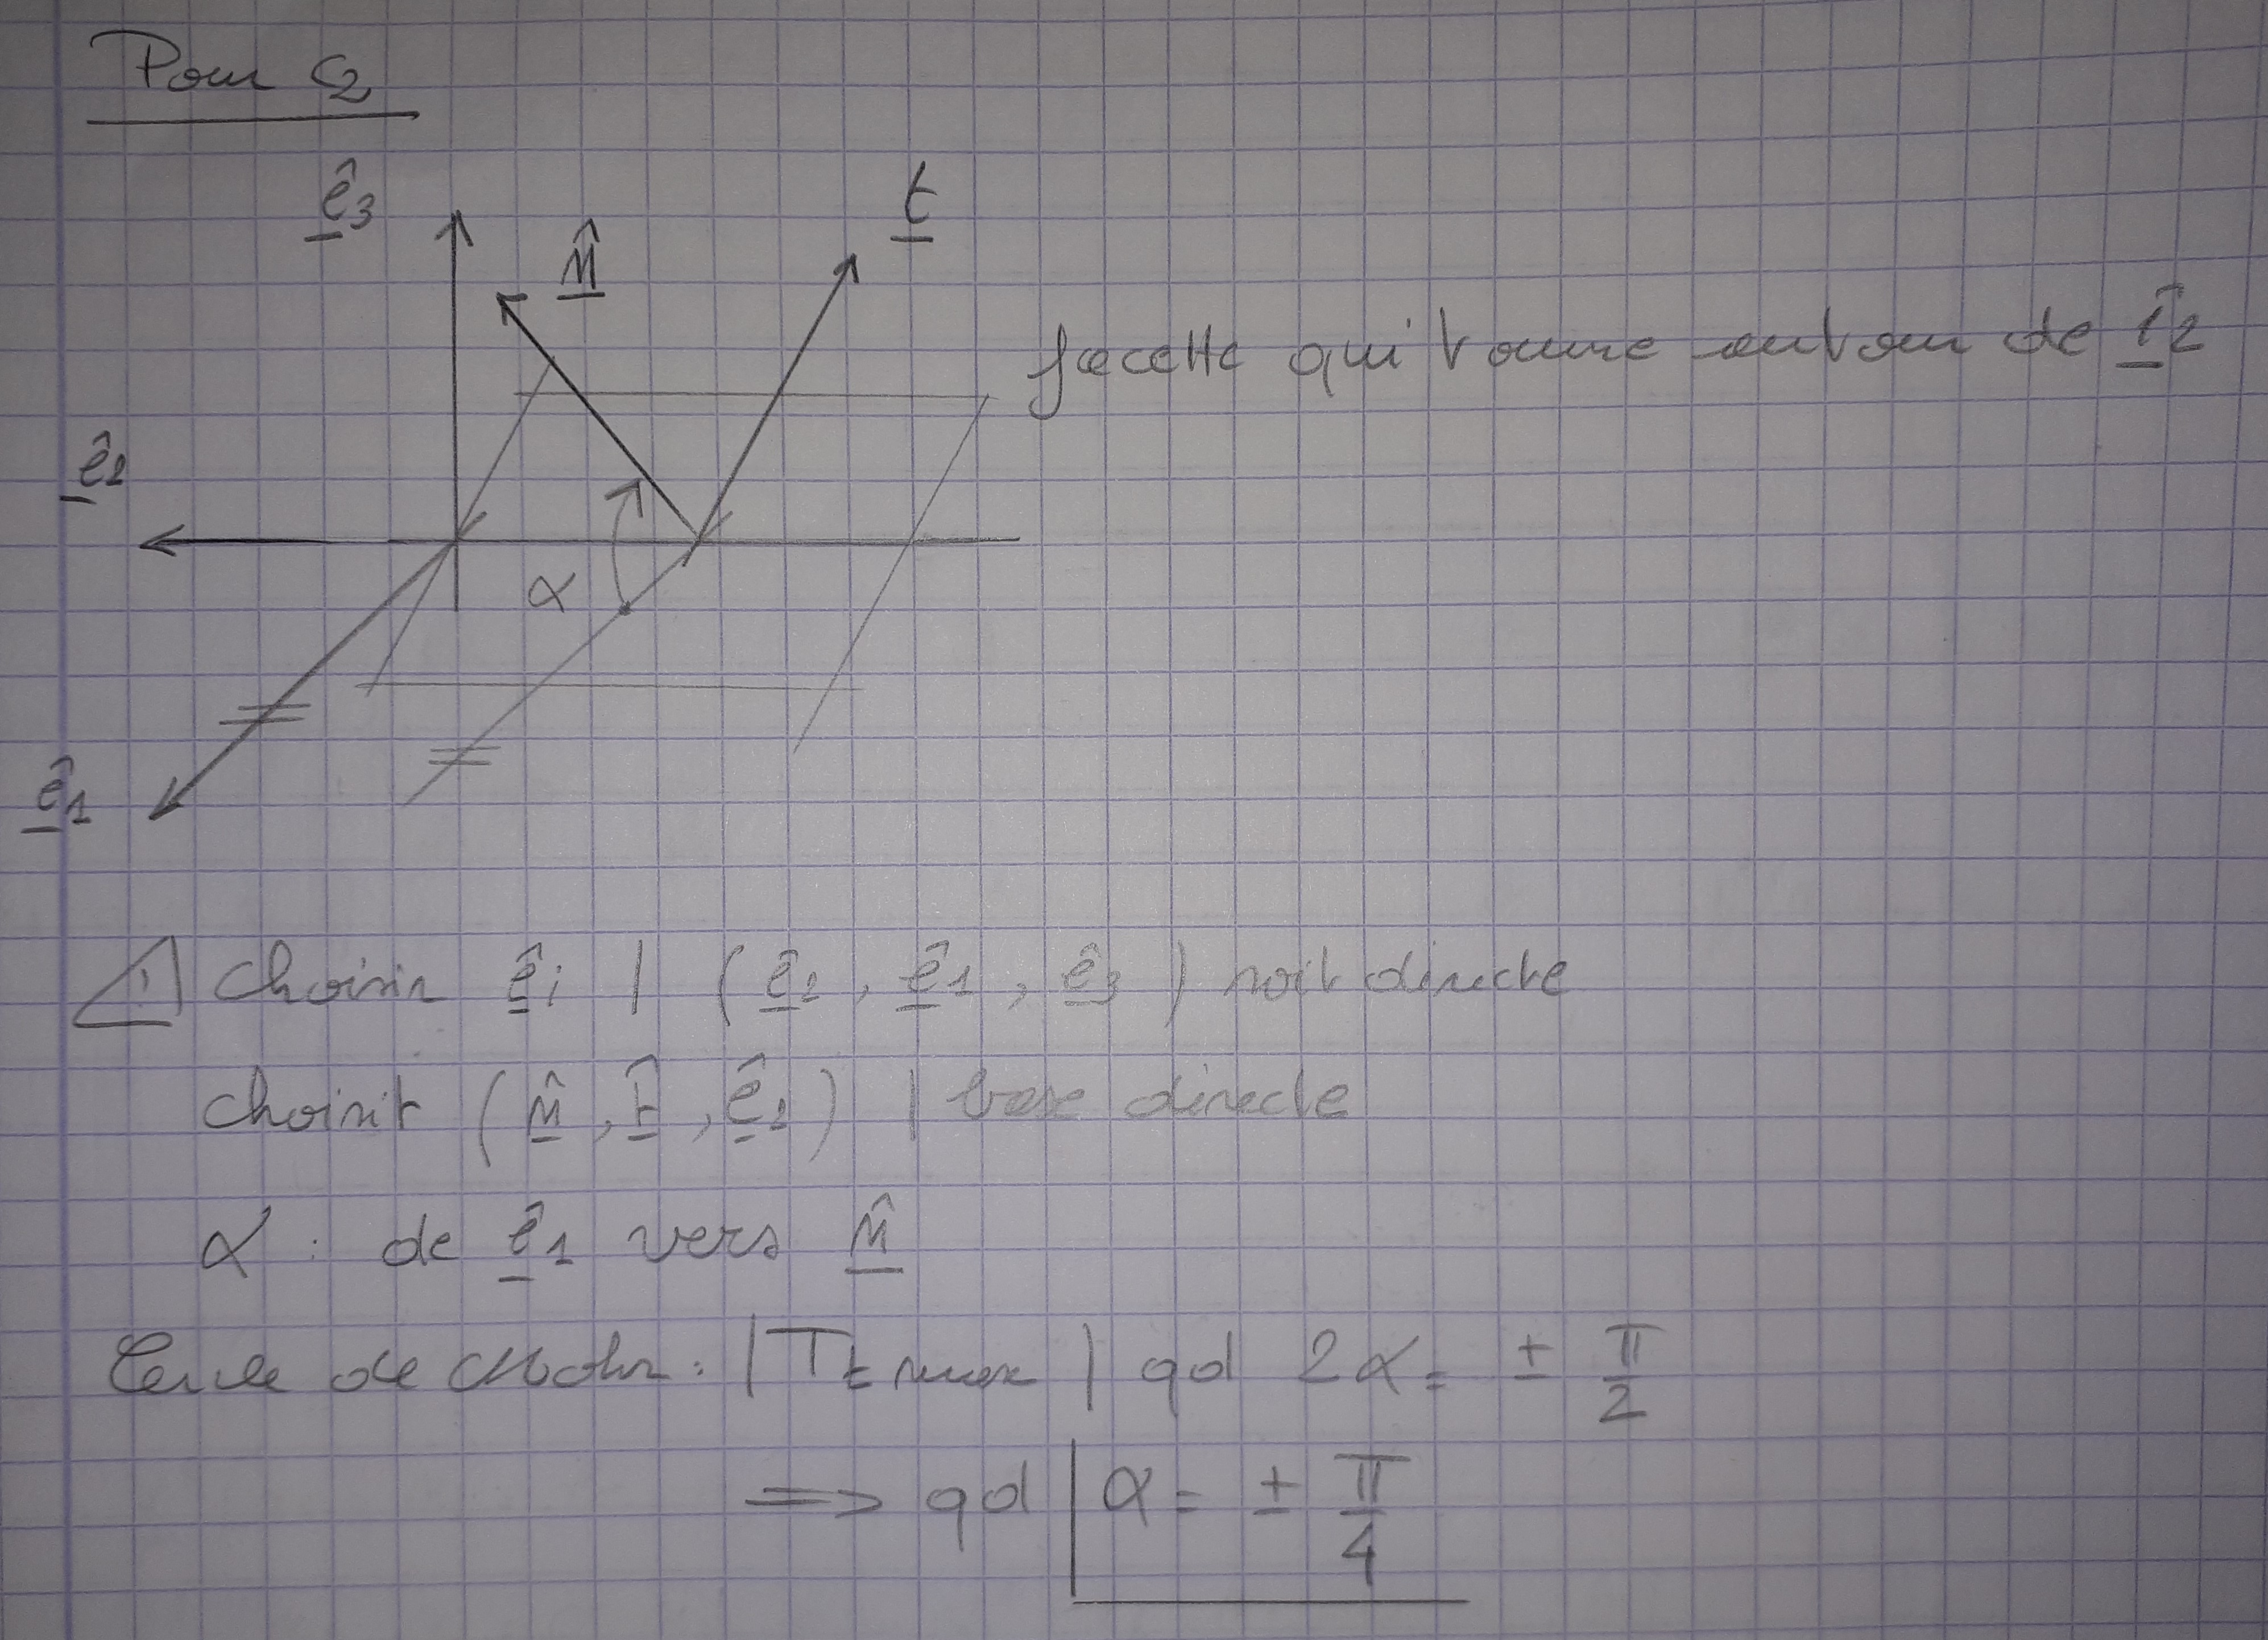
\includegraphics[width=0.9\textwidth]{MMC_Janvier_2019_Maj_Q3_Image3.jpg}
\end{center}

\end{enumerate}

\end{solution}

\section{Exercice 2}

On étudie l'écoulement stationnaire de deux fluides visqueux newtonien incompressible, indilatable et non-miscible (ne pouvant pas se mélanger) dans un canal.  Celui-ci est constitué de deux plaques planes immobiles, parallèles de longueur $L$ espacées d'une distance $2b$.

\begin{center}
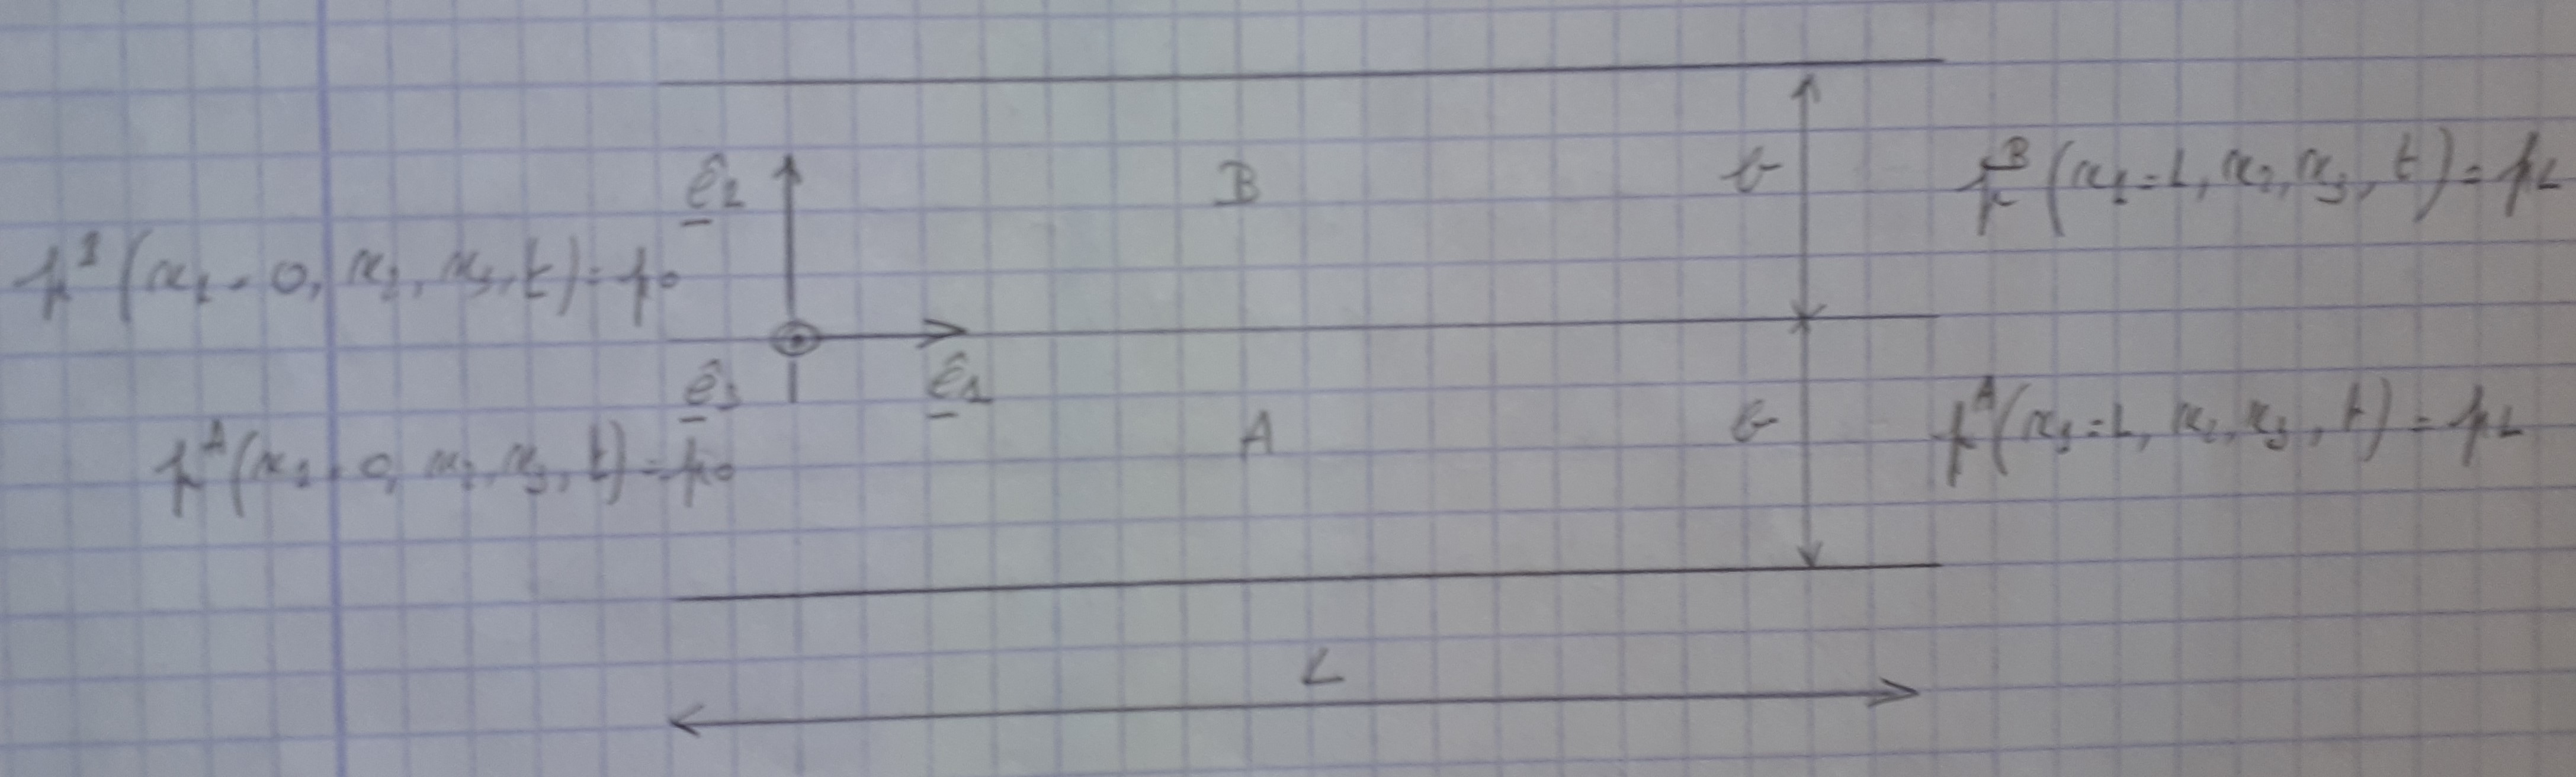
\includegraphics[width=0.9\textwidth]{MMC_Janvier_2019_Maj_Q2_Image1.jpg}
\end{center}

L'écoulement est causé par un gradient de pression constant dans le temps : la pression à l'entrée du canal est telle que $p^f(x_1=0, \ x_2, \ x_3, \ t) = p_0$ tandis que la pression à la sortie du canal vaut $p^f(x_1=L, \ x_2, \ x_3, \ t) = p_L$ avec $p_0>p_L$ et l'exposant $f$ indiquant le fluide $A$ ou $B$.  Les débits massiques de fluide $A$ et de fluide $B$ sont ajustés de sorte que le canal est rempli jusqu'à mi-hauteur de fluide $A$ tandis que le fluide $B$ occupe la moitié supérieure du canal, le fluide $A$ étant plus dense que le fluide $B$.

Les fluides sont décrots par des masses volumiques $\rho^A$ et $\rho^B$, des viscosités dynamique de cisaillement $\mu^A$ $\mu^B$, respectivement.  Ces derniers sont toutes supposées constantes.  Les plaques planes étant de très grandes dimensions, on négligera les effets se produisant aux extrémités.  Nous considérons qu'il n'y aucune force de volume agissant sur le système (donc pas de force gravitationnelle non plus.

\begin{enumerate}

\item Ecrire les conditions frontières associées au champ de vitesse.  Que doit-on notamment garantir à l'interface entre les deux fluides~?

\item En utilisant la méthode semi-inverse, obtenir la forme de champ de vitesse $v^f$ avec l'exposant $f$ indiquant le fluide $A$ ou $B$.  Veillr à justifier de façon claire et précise toutes les simplifications.

\item Sans les résoudre, obtenir les équations à résoudre pour obtenir les champs de vitesse et de pression.

\item Obtenir le champ de pression.  Commenter.

\item Obtenir le champ de vitesse pour les deux fluides.  Commenter.

\item Obtenir l'expression du tenseur des taux de déformations $\matr{D}^f$ ainsi que ses valeurs et vecteurs propres dans chacune des deux régions.

\item En exploitant les résultats obtenus à la question précédente, répondre aux questions ci-dessous en considérant $\mu^A > \mu^B$.

	\begin{enumerate}
	
	\item Au moyen d'un colorant, on dessine une croix en 		$x_2=-b/2$.  Celle-ci est initialement formée de deux segments infinitésimaux perpendiculaires de longueurs $dL_0$ orientés parallèlement aux vecteurs de base $\hat{e}_1$ et $\hat{e}_2$.  Indiquer la (les) affirmation(s) correcte(s) pour des temps courts :
	
		\begin{enumerate}	

		\item Les segments de la croix vont s'allonger.

		\item Le segment initialement aligné avec le vecteur de la base $\hat{e}_1$ va s'allonger tandis que le segment initialement aligné avec le vecteur $\hat{e}_2$ va se raccourcir.
		
		\item La longueur des segments van rester inchangée.
		
		\item L'angle $\alpha$ va augmenter.
		
		\item L'angle $\alpha$ va diminuer.
		
		\item Aucune de ces proposions. 		

		\end{enumerate}	
	 		
	\end{enumerate}

Remarque : j'ai retranscrit ici l'énoncé qui a été recopié par un autre étudiant et je n'ai pas vu l'original.  Sur la feuille, il n'y a qu'une sous-question $(a)$.  Je ne sais pas si c'est une erreur de numérotation ou bien s'il manque des sous-questions. 

\end{enumerate}

\begin{solution}

\begin{enumerate}
 
 \item 

$\vec{V}^A (x_1, x_2 = -b, x_3, t) = \vec{0}$

$\vec{V}^B (x_1, x_2 = b, x_3, t) = \vec{0}$


$\vec{V}^A (x_1, x_2 = 0, x_3, t) = \vec{V}^B (x_1, x_2 = 0, x_3, t)$

\item 

$\vec{V}^f(x_1, x_2, x_3, t)
= V^f_1(x_1, x_2, x_3, t) \ \vec{\hat{e}}_1
+ V^f_2(x_1, x_2, x_3, t) \ \vec{\hat{e}}_2
+ V^f_3(x_1, x_2, x_3, t) \ \vec{\hat{e}}_3$

Composantes

\begin{itemize}
	\item $V^f_1$ : OUI car gradient de pression suivant $\vec{\hat{e}}_1$.
	\item $V^f_2$ : NON car il n'y a rien pour faire se déplacer le fluide suivant $\vec{\hat{e}}_2$, et on fait l'hytpothèse qu'il se déplace suivant des lames horizontales. 
	\item $V^f_3$ : NON car il n'y a rien pour faire se déplacer le fluide suivant $\vec{\hat{e}}_3$ : gradient de pression, singularité, effet de bord  (plaques infinies suivant $\vec{\hat{e}}_3$). 
\end{itemize}

Dépendances de $V^f_1$

\begin{itemize}
	\item $x_1$ : NON car fluide incompressible : avec l'hytpohèse du fluide se déplaçant suivant des lames, les particules d'une lame doivent toutes se déplacer à la même vitesse, sinon elles s'accumuleraient ou s'écarteraient les unes des autres, et la masse volumique varierait.
	\item $x_2$ : OUI car vitesse nulle aux parois mais non nulle ailleurs pour qu'il y ait un débit. 
	\item $x_3$ : NON car plaque infinie dans la direction $\vec{\hat{e}}_3$ (pas d'effet de bord).
	\item $t$ : NON car stationnaire. 
\end{itemize}

$\Rightarrow \ \boxed{\vec{V}^f = V^f_1(x_2) \ \vec{\hat{e}}_1}$

$p^f = p^f(x_1, x_2, x_3, t)$

Dépendances de $p^f$

\begin{itemize}
	\item $x_1$ : OUI car gradient de pression suivant $\vec{\hat{e}}_1$.
	\item $x_2$ : NON (pour un fluide donné) car $p^f$ en $x_1=0$ et $x_1=L$ est constante pour tout $x_2$ et pour tout $x_3$.  Suppose que ça ne change pas entre $x_1=0$ et $x_1=L$ car pas de singularité (changement de géométrie). 
	\item $x_3$ : NON.  Idem $x_2$.
	\item $t$ : NON car stationnaire. 
\end{itemize}

$\Rightarrow \ \boxed{ p^f = p^f(x_1) }$

\item 

$\boxed{ \rho \fDif{\vec{V}}{t} = \rho \vec{f} - \vec {\text{grad}} \ p + \mu \Delta \vec{V}}$

$\boxed{ \matr{\sigma} = 2 \mu \matr{D} + \lambda \ \text{tr} \matr{D} \ \matr{I} - p \ \matr{I}}$

\item 

\begin{align*} 
\rho \fDif{\vec{V}}{t} &= \rho \vec{f} - \vec {\text{grad}} \ p + \mu \Delta \vec{V} \\
\rho \frac{\partial \vec{V}}{\partial t} + \rho \ \left( \matr{\text{grad}} \ \vec{V} \right) \cdot \vec{V} &= \rho \vec{f} - \vec {\text{grad}} \ p + \mu \Delta \vec{V} \\
\rho \ \begin{pmatrix} 0 & \frac{\partial V_1}{\partial x_2} \\ 0&0&0 \\ 0&0&0 \\ \end{pmatrix} \begin{pmatrix} 0 \\ V_1 \\ 0 \\ \end{pmatrix} &= \begin{pmatrix} - \frac{\partial p}{\partial x_1} \\ 0 \\ 0 \\ \end{pmatrix} + \begin{pmatrix} \mu \frac{\partial ^2 V_1}{\partial x^2_2} \\ 0 \\ 0 \\ \end{pmatrix} \\
\begin{pmatrix} 0 \\ 0 \\ 0 \\ \end{pmatrix} &= \begin{pmatrix} - \frac{\partial p}{\partial x_1} \\ 0 \\ 0 \\ \end{pmatrix} + \begin{pmatrix} \mu \frac{\partial ^2 V_1}{\partial x^2_2} \\ 0 \\ 0 \\ \end{pmatrix}
\end{align*}

$\Rightarrow \ \frac{\partial p^f}{\partial x_1} = \mu^f \frac{\partial ^2 V^f_1}{\partial x^2_2} = K^f_1$

Le premier membre est une fonction de $x_1$ et le second de $x_2$ (voir les dépendances de $p$ et $\vec{V}$ au point 1).  Les deux fonctions sont donc égales à une constante $K^f_1$.

Pour $p$ : $\frac{\partial p^f}{\partial x_1} = K^f_1 \ \Rightarrow \ p^f = K^f_1 x_1 + K^f_2$

C.L. : $p^f(x_1=0) = p^f(x_1=0) = p_0$ et $p^f(x_1=L) = p^f(x_1=L) = p_L$ pour $A$ et $B$.

$p^f_0 = K^f_2$

$p^f_l = K^f_1 \ L + p_0 \Rightarrow \ K^f_1 = \frac{p_L - p_0}{L}$

$\Rightarrow \ \boxed{ p^A = p^B = \frac{p_L - p_0}{L} x_1 + p_0} $ et $\boxed{ K^A_1 = K^B_1 = \frac{p_L - p_0}{L} }$

Commentaire : je ne sais pas exactement ce que le professeur attendait.  Voici ce à quoi me fait penser la réponse :
\begin{itemize}
\item $p^A = p^B$ semble plausible car, à l'interface au moins, les pressions statiques doivent être les mêmes (la pression statique se transmet intégralement et dans toutes les directions).
\item Les gradients de pressions sont les mêmes, mais les viscosités sont différentes. On doit donc s'attendre à ce que les vitesses soient différentes.
\end{itemize}

\item 

$\mu^f \frac{\partial^2 V^f_1}{\partial x^2_2} = K^f_1 \ \Rightarrow \ \boxed{ V^f_1 =\frac{K^f_1}{\mu^f} \frac{x^2_2}{2} + K^f_2 x_2 + K^f_3} $

On connait déjà $K^f_1$.  Il reste quatre constantes à trouver.  On a que trois conditions limites qui font intervenir les vitesses.  On peut en obtenir une quatrième en faisant intervenir les contraintes : à l'interface, les contraintes agissant sur les fluides ont la même amplitudes mais leur direction sont opposée (principe d'action-réaction).

\begin{equation*}
\begin{split}
\matr{\sigma}
&= \matr{\sigma} = 2 \mu \matr{D} + \lambda \ \text{tr} \matr{D} \ \matr{I} - p \ \matr{I} \\
&= \begin{pmatrix}
-p & \mu \frac{\partial V_1}{\partial x_2} & 0 \\
\mu \frac{\partial V_1}{\partial x_2} & -p & 0 \\
0 & 0 & -p\\
\end{pmatrix}
\end{split}
\end{equation*}

Contrainte exercée par le fluide $B$ sur le fluide $A$ :

$\vec{T}^A (x_2=0, \ \vec{\hat{n}} =\vec{\hat{e}}_2) = \matr{\sigma} \cdot \ \vec{\hat{e}}_2 = \begin{pmatrix} \mu^A \frac{\partial V^A_1}{\partial x_2} & -p^A & 0 \end{pmatrix}^T $

Contrainte exercée par le fluide $A$ sur le fluide $B$ :

$\vec{T}^B (x_2=0, \ \vec{\hat{n}} = - \vec{\hat{e}}_2) = \matr{\sigma} \cdot \ - \vec{\hat{e}}_2 = \begin{pmatrix} - \mu^B \frac{\partial V^B_1}{\partial x_2} & p^B & 0 \end{pmatrix}^T $

C.L. : $\vec{T}^A (x_2=0, \ \vec{\hat{n}} =\vec{\hat{e}}_2) = - \vec{T}^A (x_2=0, \ \vec{\hat{n}} = - \vec{\hat{e}}_2)$

\begin{align*}
\mu^A \frac{\partial V^A_1}{\partial x_2} & = \mu^B \frac{\partial V^B_1}{\partial x_2} \\
\mu^A \frac{K^A_1}{\mu^A} x_2 + \mu^A K^A_2 & = \mu^B \frac{\partial V^B_1}{\partial x_2}  x_2 + \mu^B K^A_B  \\
\mu^A K^A_2 & = \mu^B K^A_2  \\
\end{align*}

(On trouve aussi $p^A = p^B$.  Inutile ici, mais confirme le résultat obtenu au point précédent.)

Les quatres C.L. nous donnent donc ce système :

$\begin{cases}
V^A_1 (x_2=-b) = \frac{K_1}{2 \mu^A} b^2 - K^A_2 b + K^A_3 = 0 \\
V^B_1 (x_2= b) = \frac{K_1}{2 \mu^B} b^2 - K^B_2 b + K^B_3 = 0 \\
V^A_1 (x_2=0) = V^B_1 (x_2=0) = K^A_3 = K^B_3 \\
\mu^A K^A_2 = \mu^B K^A_2 \\
\end{cases}$

On trouve :

\begin{equation*}
\boxed{K^A_2 = \frac{p_0-p_L}{L} \ \frac{b}{2 \mu^A} \ \frac{\mu^A-\mu^B}{\mu^A+\mu^B}}
\end{equation*}

\begin{equation*}
\boxed{K^B_2 = \frac{p_0-p_L}{L} \ \frac{b}{2 \mu^B} \ \frac{\mu^A-\mu^B}{\mu^A+\mu^B}}
\end{equation*}

\begin{equation*}
\boxed{K^A_3 = K^B_3 = \frac{b^2 (p_0-p_1)}{L (\mu^A + \mu^B)}}
\end{equation*}

Commentaire : les profils de vitesse dans le fluide $A$ et $B$ ont la même allure, mais les vitesses sont différentes ($K^A_2 \ne K^B_2$).  Ce dernier point a été prédit à la fin de la question précédente.  Je ne trouve pas ce commentaire très intéressant, mais je ne sais pas quoi dire d'autre.  Le résultat ne me fait pas  penser à quelque chose vu au cours ou en APE.

\item 

Tenseur taux de déformation

\begin{equation*}
\boxed{ \matr{D}^f
= \frac{1}{2} \left[ \left( \matr{\text{grad}} \ \vec{V}^f \right) + \left( \matr{\text{grad}} \ \vec{V}^f \right)^T \right]
= \begin{pmatrix} 0 & D_{12}^f & 0 \\ D_{21}^f & 0 & 0 \\ 0 & 0 & 0 \\ \end{pmatrix} }
\end{equation*}

Avec

\begin{equation*}
\begin{split}
D_{12}^f = D_{21}^f
& = \frac {\partial V^f_1}{\partial x_2} \\
& = \frac {K^f_1}{\mu^f}x_2 + K^f_2 \\
& = \frac{p_L-p_0}{\mu^f L} x_2 + \frac{p_L-p_0}{L}\frac{b}{2 \mu^f} \frac{\mu^B-\mu^A}{\mu^A+\mu^B} \\
& = \boxed{ \frac{p_L-p_0}{\mu^f L} \left( x_2 + \frac{b}{2} \  \frac{\mu^B-\mu^A}{\mu^A+\mu^B} \right) } 
\end{split}
\end{equation*}

Valeurs propres

$\text{det} \left( \matr{D}^f - \lambda \matr{I} \right)
= \begin{vmatrix} -\lambda & D^f_{12} & 0 \\ D^f_{12} & -\lambda & 0 \\ 0 & 0 & -\lambda \\ \end{vmatrix}
= - \lambda \left( \lambda^2 - D^f_{12} \right)$

$\Rightarrow \ \boxed{ \lambda_1 = 0 \ \text{et} \ \lambda_{2,3} = \pm D^f_{12} }$ 

Vecteurs propres associés à $\lambda_1 = 0$

$
\begin{pmatrix} 0 & D_{12} & 0 \\ D_{12} & 0 & 0 \\ 0 & 0 & 0 \\ \end{pmatrix}
\ \begin{pmatrix} x_1 \\ x_2 \\ x_3 \\ \end{pmatrix}
= \begin{pmatrix} 0 \\ 0 \\ 0 \\ \end{pmatrix}
\ \Rightarrow \ \boxed { \vec{\hat{c}}_1
= \begin{pmatrix} 0 \\ 0 \\ 1 \\ \end{pmatrix} }
$

Vecteurs propres associés à $\lambda_2 = D^f_{12}$

$
\begin{pmatrix} - D^f_{12} & D_{12} & 0 \\ D_{12} & - D^f_{12} & 0 \\ 0 & 0 & -D^f_{12} \\ \end{pmatrix}
\ \begin{pmatrix} x_1 \\ x_2 \\ x_3 \\ \end{pmatrix}
= \begin{pmatrix} 0 \\ 0 \\ 0 \\ \end{pmatrix}
\ \Rightarrow \ \vec{c}_2
= \begin{pmatrix} 1 \\ 1 \\ 0 \\ \end{pmatrix}
\ \Rightarrow \ \boxed { \vec{\hat{c}}_2
= \begin{pmatrix} \frac{\sqrt{2}}{2} \\ \frac{\sqrt{2}}{2} \\ 0 \\ \end{pmatrix} }
$

Vecteurs propres associés à $\lambda_3 = - D^f_{12}$

$
\begin{pmatrix} D^f_{12} & D_{12} & 0 \\ D_{12} & D^f_{12} & 0 \\ 0 & 0 & D^f_{12} \\ \end{pmatrix}
\ \begin{pmatrix} x_1 \\ x_2 \\ x_3 \\ \end{pmatrix}
= \begin{pmatrix} 0 \\ 0 \\ 0 \\ \end{pmatrix}
\ \Rightarrow \ \vec{c}_3
= \begin{pmatrix} 1 \\ - 1 \\ 0 \\ \end{pmatrix}
\ \Rightarrow \ \boxed { \vec{\hat{c}}_3
= \begin{pmatrix} \frac{\sqrt{2}}{2} \\ - \frac{\sqrt{2}}{2} \\ 0 \\ \end{pmatrix} }
$

Remarque : j'ai normé les vecteurs propres et j'ai choisi $\vec{\hat{c}}_3$ pour que la base des vecteurs propres $\left( \vec{\hat{c}}_1, \ \vec{\hat{c}}_2, \ \vec{\hat{c}}_3 \right)$ soit directe ($\vec{\hat{c}}_3 = \vec{\hat{c}}_1 \wedge \vec{\hat{c}}_2$).  Je ne pense pas que c'était obligatoire car on ne demandait que les vecteurs propres, pas d'en faire une base orthonormée directe.  Mais ça permettait de vérifier facilement qu'il n'y avait pas d'erreur dans les calculs : comme $( \matr{D} )$ est symmétrique, ses vecteurs propres sont orthogonaux entre eux et peuvent former une base orthonormée.

\item 

En $x_2 = -b/2$, on est dans le fluide $A$.

Taux d'allongement dans la direction de $\vec{\hat{e}}_1$ et de de $\vec{\hat{e}}_2$ :

\begin{equation*}
\frac{1}{dl} \ \fDif{dl}{dt} \left( \vec{\hat{e}}_1 , \ \vec{\hat{e}}_1 \right) 
= \matr{D}^A \ \left( \vec{\hat{e}}_1 , \ \vec{\hat{e}}_1 \right)
= \vec{\hat{e}}_1 \cdot \matr{D}^A \cdot \vec{\hat{e}}_1
= D^A_{\vec{1} \vec{1}}
= 0
\ (\text{pas de sommation sur }1)
\end{equation*}

\begin{equation*}
\frac{1}{dl} \ \fDif{dl}{dt} \left( \vec{\hat{e}}_2 , \ \vec{\hat{e}}_2 \right) 
= \matr{D}^A \ \left( \vec{\hat{e}}_2 , \ \vec{\hat{e}}_2 \right)
= \vec{\hat{e}}_2 \cdot \matr{D}^A \cdot \vec{\hat{e}}_2
= D^A_{\vec{2} \vec{2}}
= 0
\ (\text{pas de sommation sur }2)
\end{equation*}

La longueur des segments est donc inchangée.  Propositions $i$ et $ii$ : fausses, proposition $iii$ : vraie.

Taux de glissement des deux directions perpendiculaires de $\vec{\hat{e}}_1$ et de $\vec{\hat{e}}_2$ :

$\fDif{\theta}{t} (\vec{\hat{e}}_2, \ \vec{\hat{e}}_2)
= 2 \ \matr{D}^A \ \left( \vec{\hat{e}}_1 , \ \vec{\hat{e}}_2 \right)
= 2 \ \vec{\hat{e}}_1 \cdot \matr{D}^A \cdot \vec{\hat{e}}_2
= 2 \ D^A_{12}
= 2 \ \frac{p_L-p_0}{\mu^A L} \left( x_2 + \frac{b}{2} \  \frac{\mu^B-\mu^A}{\mu^A+\mu^B} \right)
$

En $x_2 = -b/2$ : $\fDif{\theta}{t} > 0$

Remarque : je ne sais pas conclure à l'aide de cette formule car je n'ai pas bien compris la convention utilisée pour mesurer l'angle $\theta$.  Mais comme la vitesse du fluide augmente lorsque l'on s'écarte des parois, on peut s'attendre à ce que l'angle $\alpha$ diminue.  Donc, proposition $(\vec{\hat{e}}_2, \ \vec{\hat{e}}_2) = 2 \frac{b \left(p_0-p_L \right)}{L \left(\mu^A + \mu^B\right)}$ $v$ correcte, propositions $iv$ et $vi$ fausses.

\begin{center}
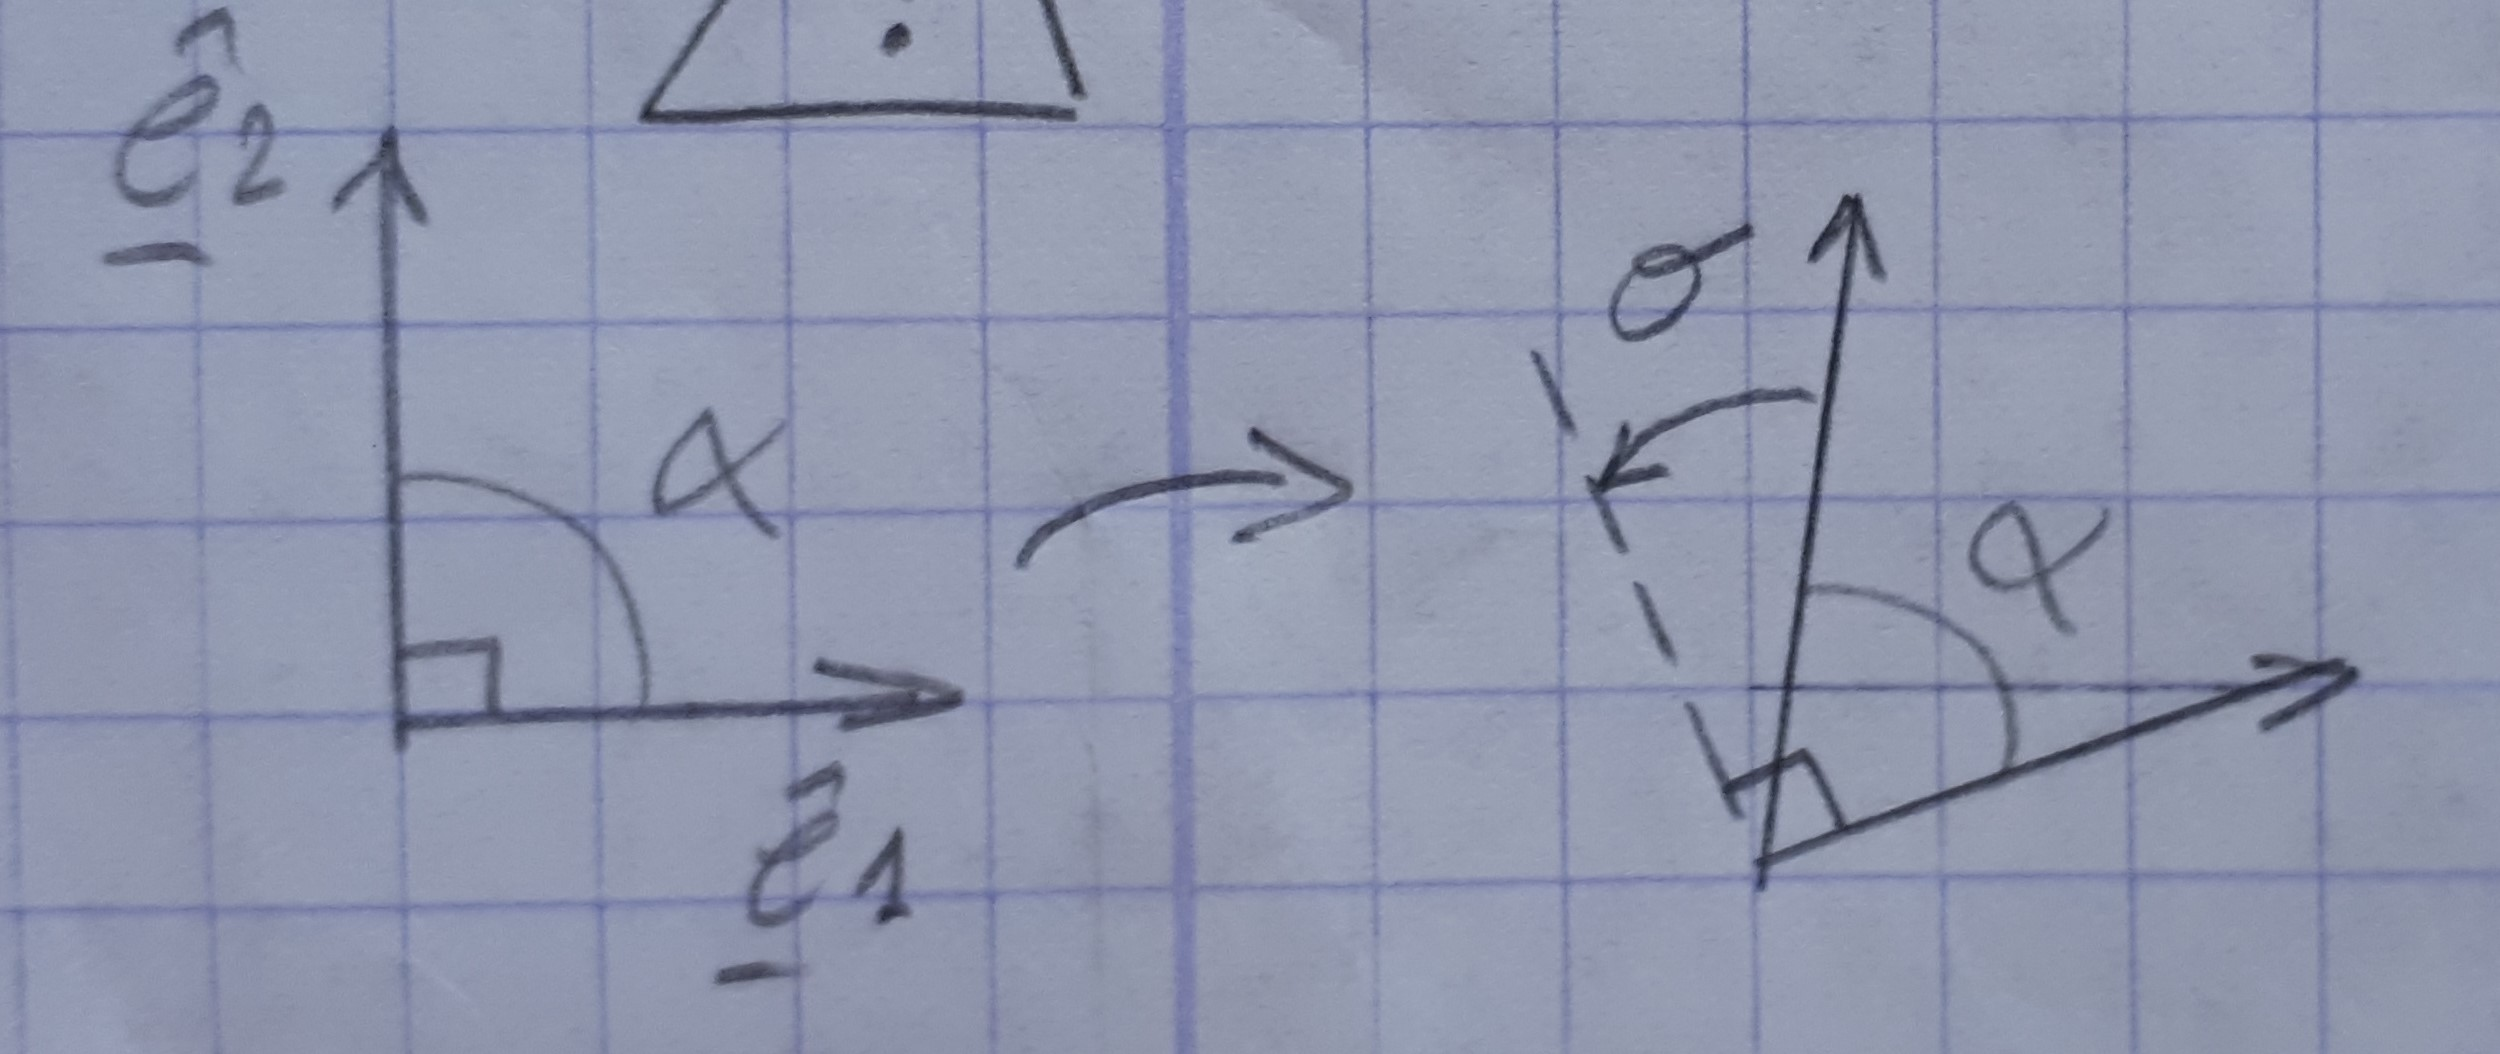
\includegraphics[width=0.9\textwidth]{MMC_Janvier_2019_Maj_Q2_Image2.jpg}
\end{center}

\begin{center}
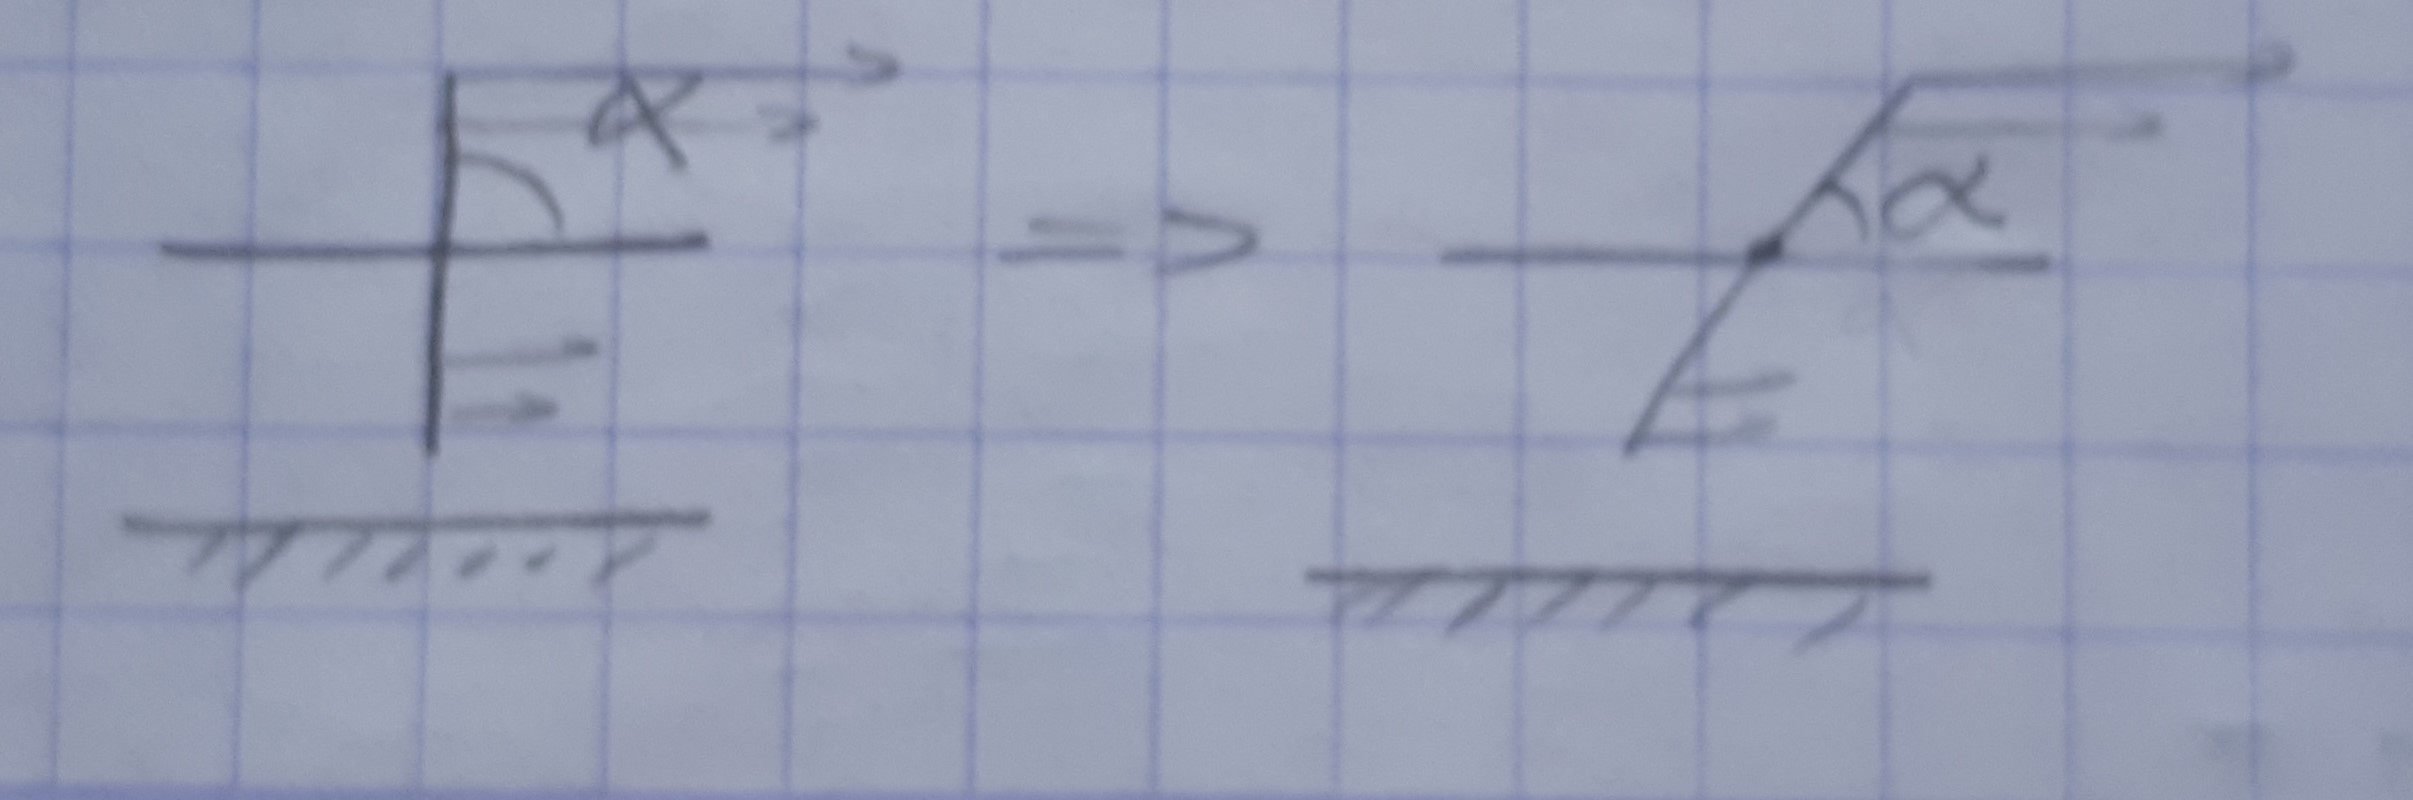
\includegraphics[width=0.9\textwidth]{MMC_Janvier_2019_Maj_Q2_Image3.jpg}
\end{center}

\end{enumerate}

\end{solution}

\end{document}
